\documentclass[addpoints,12pt]{exam}

\usepackage{amsmath, amsfonts, amssymb,tikz}

% --- Header and Footer Setup ---
\pagestyle{headandfoot}
\firstpageheader{Comp Math}{Third Homework}{September 16, 2026}
\runningheader{Comp Math}{Third Homework, Page \thepage\ of \numpages}{}
\firstpagefooter{}{}{}
\runningfooter{}{}{Page \thepage}

\begin{document}

\begin{center}
    \textbf{\Large Homework \#3} \\
    \vspace{0.1in}
    \textbf{\large Logic}
\end{center}

\vspace{0.3in}

\begin{questions}
\question Let A = $\{1, 3, 12, 35\}, B = \{3, 7, 12, 20\}$, and $C = \{x |$ x is a prime
number$ \}$. List the elements of the following sets. Are any of the sets
below disjoint from any of the others? Are any of the sets below
subsets of any others?
\begin{parts}
\part $A \cap B$

$\{$3,12$\}$

\part $(A \cup B) \setminus C$

$\{$1,3,7,12,20,35$\}$

\part $A \cup (B \setminus C)$

$\{$1,3,12,20,35$\}$

\end{parts}


\question Use any method you wish to verify the following identities:
\begin{parts}
    \part $(A \setminus B) \cap C = (A \cap C) \setminus B$

        Conditions for membership on the LHS: 

        $(A \setminus B) \cap C \implies (x \in A \land x \notin B) \land (x \in C) $

        Conditions for membership on the RHS: 

        $(A \cap C) \setminus B \implies (x \in A \land x \in C) \land (x \notin B)$

        The and operator is associative, therefore the expressions are equivalant. 

    \part $(A \cap B) \setminus B = \emptyset$

        Conditions for membership on the LHS: 

        $(A \cap B) \setminus B \implies (x \in A \land x \in B ) \land x \notin B$

        $x \in B  \land x \notin B$ is a contradiction, there is no element that is in B and not in B, so it equalts the empty set 

    \part $(A \setminus B) \setminus B = (A \cap B)$

        Conditions for membership on the LHS: 

        $(A \setminus B) \setminus B \implies (x \in A \land x \notin B) \land x \notin B $

        The last one is redundant and already imples that any element must be in A and not in B, which is the definition of a set difference.
\end{parts}

\question Use a Venn Diagram to show the associativity of the Symetric Difference
\begin{center}
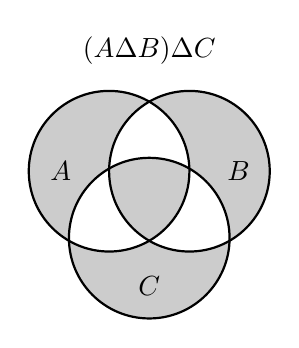
\begin{tikzpicture}[scale=0.85]
    % --- Left Diagram: (A \Delta B) \Delta C ---
    % Path definitions for circles
    \def\circleA{(0,0) circle (1.2cm)}
    \def\circleB{(1.2,0) circle (1.2cm)}
    \def\circleC{(0.6,-1) circle (1.2cm)}

    % Even Odd Rule fills regions belonging to an ODD number of circles
    \begin{scope}
        \fill[gray!40, even odd rule] \circleA \circleB \circleC;
    \end{scope}
    
    % Draw Outlines
    \draw[thick] \circleA node[left=10pt] {$A$};
    \draw[thick] \circleB node[right=10pt] {$B$};
    \draw[thick] \circleC node[below=10pt] {$C$};
    \node at (0.6, 1.8) {\textbf{$(A \Delta B) \Delta C$}};
\end{tikzpicture}
\qquad
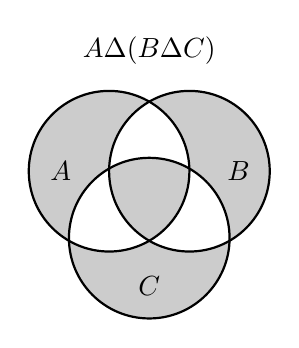
\begin{tikzpicture}[scale=0.85]
    % --- Right Diagram: A \Delta (B \Delta C) ---
    \def\circleA{(0,0) circle (1.2cm)}
    \def\circleB{(1.2,0) circle (1.2cm)}
    \def\circleC{(0.6,-1) circle (1.2cm)}

    \begin{scope}
        \fill[gray!40, even odd rule] \circleA \circleB \circleC;
    \end{scope}
    
    % Draw Outlines
    \draw[thick] \circleA node[left=10pt] {$A$};
    \draw[thick] \circleB node[right=10pt] {$B$};
    \draw[thick] \circleC node[below=10pt] {$C$};
    \node at (0.6, 1.8) {\textbf{$A \Delta (B \Delta C)$}};
\end{tikzpicture}
\end{center}

This makes sense, as the symetric difference operator essentialy acts like the XOR, so only items that are not in either set get left. And we aslo know that XOR is associative as well, so this holds up.

\question Analyze the logical forms of the following statements:
\begin{parts}
\part Mary will sell her house only if she can get a good price and find a
nice apartment.

P = Mary will sell her house

Q = She gets a good price

R = She finds a nice apartment 

$P \implies Q \land R $



\part Having both a good credit history and an adequate down payment is a
necessary condition for getting a mortgage.

P = Getting a mortgage  

Q = Having a good Credit history

R = Having an adequate down payment

$P \implies Q \land R $

\part John will drop out of school, unless someone stops him. (Hint: First
try to rephrase this using the words if and then instead of unless.)


P = John Drops out 

Q = Someone stops him

$\lnot P \implies Q$

\part If x is divisible by either 4 or 6, then it isn't prime.

P = x is Prime 

Q = $x\  |\  4$

R = $x\ |\  6$

$Q  \vee R \implies \lnot P$

\end{parts}

\question  Show that $(P \rightarrow Q) \land (Q \rightarrow R)$ is equivalent to $(P \rightarrow R) \land [(P \iff
Q)\vee (R \iff Q)]$.


\begin{table}[h!]
\centering
\caption{Truth Table Verification of Logical Equivalence}
\label{tab:truth_table}
\begin{tabular}{|c|c|c||c|c|c||c|c|c|c|}
\hline
$P$ & $Q$ & $R$ & $P \rightarrow Q$ & $Q \rightarrow R$ & \textbf{LHS} & $P \rightarrow R$ & $P \iff Q$ & $R \iff Q$ & \textbf{RHS} \\ \hline
T   & T   & T   & T                 & T                 & \textbf{T}   & T                 & T          & T          & \textbf{T}   \\ \hline
T   & T   & F   & T                 & F                 & \textbf{F}   & F                 & T          & F          & \textbf{F}   \\ \hline
T   & F   & T   & F                 & T                 & \textbf{F}   & T                 & F          & F          & \textbf{F}   \\ \hline
T   & F   & F   & F                 & T                 & \textbf{F}   & F                 & F          & T          & \textbf{F}   \\ \hline
F   & T   & T   & T                 & T                 & \textbf{T}   & T                 & F          & T          & \textbf{T}   \\ \hline
F   & T   & F   & T                 & F                 & \textbf{F}   & T                 & F          & F          & \textbf{F}   \\ \hline
F   & F   & T   & T                 & T                 & \textbf{T}   & T                 & T          & F          & \textbf{T}   \\ \hline
F   & F   & F   & T                 & T                 & \textbf{T}   & T                 & T          & T          & \textbf{T}   \\ \hline
\end{tabular}
\end{table}

\question Which of the following formulas are equivalent?
\begin{parts}
\part $P \rightarrow (Q \rightarrow R) \equiv \lnot P \lor \lnot Q \lor R$

\part $Q \rightarrow (P \rightarrow R) \equiv \lnot Q \lor \lnot P \lor R \equiv \lnot P \lor \lnot Q \lor R$

\part $(P \rightarrow Q) \lor (P \rightarrow R) \equiv (\lnot P \lor Q) \lor (\lnot P \lor R) \equiv \lnot P \lor \lnot Q \lor R$

\part $(P \land Q) \rightarrow R \equiv \lnot (P \land Q) \lor R \equiv \lnot P \lor \lnot Q \lor R$

\part $P \rightarrow (Q \land R) \equiv \lnot P \lor (Q \land R) \equiv (\lnot P \lor Q) \land (\lnot P \lor R)$
\end{parts}

{(a), (b), (c), and (d)} are all logically equivalent to each other.


\end{questions}
\end{document}